\documentclass[article,	12pt,	oneside, a4paper,	english, brazil, sumario=tradicional, section=TITLE]{abntex2}

\usepackage{forscience}
\usepackage{xcolor,colortbl}


\begin{document}
\linenumbers % enumeração das linhas do trabalho

\vspace{1cm}
\begin{center}
\textbf{COMPORTAMENTO DE REDES NEURAIS ARTIFICIAIS MLP PARA CLASSFICAÇÃO DE QUESTÕES DO ENEM BASEADO EM TRI}
\end{center}\vskip 0.5em                % Espaço vertical após o título.

\begin{center}
\textbf{RESUMO}
\end{center}
\noindent O Exame Nacional do Ensino Médio (ENEM) ganha a cada ano mais importância, substituindo vestibulares tradicionais. Com isso, o desenvolvimento de ferramentas que auxiliem a preparação dos estudantes é de grande importância. Muitos simulados são feitos de forma praticamente aleatória, com questões escolhidas sem critério.  Neste contexto, este trabalho apresenta o desenvolvimento de uma rede neural para classificação de questões do ENEM, com base nos parâmetros de Teoria de Resposta ao Item. Para isso, será utilizado o algoritmo \textit{k-means} para gerar um \textit{dataset} contendo a classificação dessas questões em 3 grupos: Fáceis, Médias e Difíceis. Com esse \textit{dataset} uma rede neural será treinada para realizar a classificação das questões e verificar os resultados. Dessa maneira esse estudo contribui permitindo a elaboração de simulados de forma balanceada. Além disso, após o treinamento da rede a mesma será capaz de realizar a classificação de novas questões com base no TRI. Caso o \textit{k-means} continuasse a ser utilizado a classificação teria que ser feita novamente caso novas questões fossem adicionadas a base de questões. A rede desenvolvida teve praticamente o mesmo desempenho que o \textit{k-means} na tarefa de classificação, isso mostra a capacidade que as rede neurais possuem de classificação.\par \vspace{1.0em}

\noindent\textbf{Palavras-chave: } Enem. Algoritmos de classificação. Teoria de Resposta ao Item.
\par \vspace{1.0em}
\OnehalfSpacing % a partir desse pontos o espaçamento entre linhas será de 1,5 cm.

\section{INTRODUÇÃO}

Neste capítulo será apresentado uma introdução a assuntos que são relevantes para o entendimento do trabalho proposto. A ordem de apresentação do capítulo será a seguinte: Contextualização, Justificativa, Objetivos e Contribuições.

\subsection{Contextualização}

Em 2009 o ENEM adotou o sistema de Teoria de Resposta ao Item (TRI) que substituiu a Teoria Clássica dos Testes (TCT), o qual considerava somente a quantidade de acertos e erros para o cálculo da nota. Com o passar dos anos o ENEM ganhou espaço em meio aos tradicionais vestibulares que eram aplicados por cada instituição. Ainda assim, atualmente existem poucas ferramentas que utilizam TRI para auxiliar na preparação dos estudantes, por exemplo, grande parte dos simulados feitos em escolas e cursinhos preparatórios para o ENEM são feitos por professores que montam as provas escolhendo questões de maneira aleatória. Entretanto, essa não é a maneira ideal de se montar um caderno de provas, já que os parâmetros do TRI de cada questão podem ser calculados com base nos dados de acertos e erros referentes a questão. E com base nesses parâmetros é possível classificar as questões em grupos de dificuldade, possibilitando a geração de simulados de forma inteligente.

O presente trabalho é apresentado neste contexto, onde a construção dos cadernos de questões para simulações do ENEM é feita de forma balanceada, baseando-se nos parâmetros de cada questão e não aleatoriamente. Na próxima seção é abordada a justificativa da pesquisa.

\subsection{Justificativa e proposta}
O ENEM é utilizado por 1434 instituições de ensino superior no Brasil para selecionar os candidatos às vagas, sendo o maior vestibular do país \cite{guiaEstudante}. Diante disso, o desenvolvimento de uma ferramenta dotada dos recursos oferecidos por redes neurais para classificar questões em grupos de dificuldade é um grande passo para evolução dos métodos de ensino e de métodos de avaliação que se baseiam no TRI. Dessa maneira, estudantes podem fazer sua preparação de forma orientada, tendo a possibilidade de iniciar seus estudos com questões de dificuldade mais baixa e conforme forem evoluindo com os estudos elevem os níveis de dificuldade das questões.

 
\subsection{Objetivos}
Este estudo propõe atender ao objetivo geral e aos objetivos específicos descritos a seguir.

\subsubsection{Objetivo Geral}
Propor o desenvolvimento de uma rede neural que seja capaz de classificar questões com base nos parâmetros de Teoria de Resposta ao Item.

\subsubsection{Objetivos específicos}
São objetivos específicos deste trabalho:
\begin{enumerate}

\item Possibilitar a geração simulados com base na dificuldade das questões e não aleatoriamente.

\item Verificar a capacidade das redes neurais em classificação de questões com base nos parâmetros de Teoria de Resposta ao Item.
\end{enumerate}

\subsection{Contribuições}
Espera-se que com o desenvolvimento do trabalho proposto que simulados possam ser gerados com base nos grupos de dificuldade das questões e não de forma aleatória. Com isso, é possível por exemplo avaliar se alunos estão errando questões consideradas fáceis e buscar a melhor forma de corrigir as deficiências no ensino. Aliado a isso, avaliar a capacidade das RNAs na classificação de questões e contribuir para trabalhos futuros relacionados a área.

Na seção a seguir serão tratados tópicos importantes para o entendimento do trabalho.
\section{DESENVOLVIMENTO}
Alguns pontos fundamentais para o entendimento da dinâmica da classificação de questões são discutidos na sequência. A ordem de apresentação do capítulo é a seguinte: Teoria de Resposta ao Item, Rede Neural Artificial, Perceptron, MLP e Trabalhos Relacionados.

\subsection{Referencial Teórico}

\subsubsection{Algoritmos de classificação}	
O reconhecimento de padrões (RP) é uma tarefa da qual nós, humanos, dependemos ao longo dos anos para sobreviver. É algo que nos trouxe vantagem competitiva no meio natural e, por isso, sabemos que seu uso pode resolver diversos tipos de problema e ser útil nas mais variadas situações. O reconhecimento de padrões, por suas vantagens, tem sido utilizado nos últimos anos como estratégia para melhorar a qualidade do serviço produzido por máquinas. É um subtópico da aprendizagem de máquina, que tem como objetivo classificar objetos em categorias. Para isso análise estatística das aglomerações de dados são realizadas. (PASSOS, 2005). RP pode ser aplicado a processamento de sinais e imagens, sistemas adaptativos, mineração de dados e outros contextos onde existam informações disponíveis e passíveis de análise (PASSOS, 2005).

Realizar o reconhecimento de padrões em determinados datasets pode não ser uma tarefa trivial, por isso foram criados os algoritmos de classificação. Eles tem como objetivo dividir os elementos da amostra em grupos (clusters), de forma que os elementos de um mesmo grupo tenham características semelhantes entre si \citeonline{mingoti}.

\subsubsection{Teoria de Resposta ao Item}
No ano de 2009 o TRI foi implantado no cálculo das notas do ENEM, deixando para trás a Teoria Clássica dos Testes (TCT) que faz o cálculo das notas levando em consideração apenas a quantidade de acertos. Segundo \citeonline{tavares} a Teoria de Resposta ao Item (TRI) é um conjunto de modelos matemáticos que representam a chance do indivíduo que está respondendo à questão acertá-la com base nos parâmetros da mesma e da sua habilidade. Ou seja, o modelo é baseado em uma função crescente que indica que quanto maior o traço latente (habilidade), maior a chance de acerto no item \citeonline{moreira}.                     

Entre as principais vantagens da TRI em relação a TCT é que ela permite que duas populações sejam comparadas, desde que as provas tenham itens em comum \citeonline{moreira}. Com TRI isso é possível de ser feito graças ao modelo teórico baseado nos itens e não nos testes, onde cada resposta correta apresenta uma informação sobre o traço latente \citeonline{castro}.                                  

As funções de probabilidade do tipo logístico são as mais utilizadas atualmente e dão origem aos modelos logísticos \citeonline{castro}. No presente trabalho será trabalhado o modelo 3PL, que descreve a relação entre a habilidade do indivíduo examinado e a probabilidade de uma resposta correta considerando três parâmetros: dificuldade, discriminação e casualidade \citeonline{moreira}

\subsubsection{Rede Neural Artificial}
A ideia da construção de tecnologias autônomas, que sejam dotadas de inteligência, sempre foi um dos grandes desafios no âmbito de desenvolvimento tecnológico na história da humanidade. Essa ideia surgiu através da necessidade de solução de problemas em diversas áreas do conhecimento, desde a microbiologia até as engenharias de um modo geral e que eram muito difíceis ou exarcebadamente complexos para as capacidades dos seres humanos. A Rede Neural Artificial (RNA) é uma dessas tecnologias, e através de modelos computacionais simula o funcionamento do sistema nervoso dos seres vivos. As primeiras publicações sobre RNA começaram em meados de 1940 com os trabalhos de McCulloch \& Pitts (1943), contudo em 1990 o tema começou a ser fortemente pesquisado devido aos grandes avanços da computação e posteriormente devido a revolução da Internet e consequentemente o \textit{Big Data}.

\subsubsection{\textit{Multilayer Perceptron}}
Segundo \citeonline{silva} o \textit{Perceptron}, idealizado por Rosenblatt(1958), é a forma mais simples de configuração de uma rede neural artificial, cujo propósito focava em implementar um modelo computacional inspirado na retina, objetivando-se então um elemento de percepção eletrônica de sinais. Uma de suas aplicações consistia em identificar padrões geométricos. A concepção inicial de uma rede \textit{perceptron} consistia em um conjunto de entradas com seus respectivos pesos sinápticos, um único neurônio e uma única saída.

As redes \textit{perceptron} de múltiplas camadas (PMC) também conhecidas como \textit{Multilayer Perceptron} (MLP), são caracterizadas pela presença de pelo menos uma sub camada intermediária (escondida) de neurônios, situada entre a camada de entrada e a respectiva camada neural de saída \citeonline{silva}.
O algoritmo das PMC é dividido em dois: algoritmo de treinamento e a algoritmo de classificação. No algoritmo de treinamento utiliza-se a ideia de \textit{backpropagation}, dividindo a execução na parte \textit{feedforward} e \textit{backward}. A fase \textit{feedforward} é o próprio algoritmo de classificação, onde a saída de cada neurônio servirá como uma das entradas da próxima camada. A parte \textit{backward} caracteriza-se por repropagar as classificações da rede através de um ajuste de pesos, baseado em equações matemáticas e na classificação advinda da fase \textit{feedforward}. 

Na seção a seguir serão apresentados trabalhos relacionados com o trabalho e contribuiram para o seu desenvolvimento.

\section{TRABALHOS RELACIONADOS}

Para o desenvolvimento do trabalho foram realizadas buscas por trabalhos relacionados, para desenvolvimento do embasamento teórico  e metodológico. A seguir seguem alguns trabalhos relacionados que contribuem para a pesquisa.

No trabalho de \citeonline{sancineto2005impacto} foi realizado um estudo sobre a quantidade mínima de amostras necessária para utilização da Teoria de Resposta ao Item. Para isso, foram criadas 9 amostras de tamanhos diferentes, a partir de uma base de 44 mil respostas de estudantes. Segundo os autores é possível concluir que, amostras com 100 pessoas são instáveis, se tornando estáveis com amostras a partir de 200 pessoas. Com um dataset de 500 sujeitos é possível obter um resultado bem mais próximo em comparação com a amostra completa, sendo que com 20 mil estudantes é praticamente igual aos resultados obtidos com a amostra total.

Existem alguns programas que podem ser utilizados para do cálculo de TRI, como o BILOG-MG que é um sistema licenciado e o R \cite{rprogram} que é livre. \citeonline{barroso2012comparaccoes} desenvolveram uma comparação entre os resultados obtidos com a utilização dos sistemas. Para isso, utilizaram 25 questões de matemática e português, que já tinham seus parâmetros calibrados. Para realização dos cálculos foram escolhidos 364 alunos da 5º e 9º série de forma aleatória, que tinham suas habilidades conhecidas. Com essa habilidade foi calculada a probabilidade de cada aluno acertar as questões e após esse processo foi utilizada a distribuição de Bernoulli para gerar a provável resposta de cada aluno a cada questão. As habilidades calculadas pelos sistemas foram parecidas. Ocorreram algumas divergências na estimação de alguns parâmetros, mas, na grande maioria as diferenças foram pequenas. Diante disso, o R é uma ótima ferramenta para fazer análises de TRI.

\citeonline{castro} realizou o cálculo dos parâmetros de TRI com a utilização do pacote ltm do R, com a máxima verosimilhança e com o método “dos intervalos”, utilizando os microdados disponibilizados pelo INEP. Segundo a conclusão dos autores, o método dos intervalos é o mais simples para ser implementado, entretanto é menos preciso. O método da máxima verosimilhança foi o mais eficiente para reproduzir as notas do ENEM. Já pacote ltm foi o que conseguiu o melhor resultado na estimação dos parâmetros do TRI.

\citeonline{dosteoria} utilizaram o programa R, que é um software livre, para realizar o cálculo da TRI. Para isso eles selecionaram a base de dados da SARESP para realização do procedimento. Ela possui uma amostra de 3 testes (manhã, tarde e noite) de Língua Portuguesa, que foram aplicados para alunos do ensino médio. Existem no R alguns pacotes para cálculo de TRI, como o ltm \cite{ltm}. No estudo foi feita a análise com o pacote ltm, com o modelo de 2 e 3 parâmetros. Os autores concluíram que até o término do trabalho ainda existiam algumas funções que poderiam ser desenvolvidas para facilitar os trabalhos com o R. Não existe, por exemplo, funções para estimação de parâmetros em modelos normais. Além dos pacotes utilizados no estudo Andrade e Anjos ainda citam outro importante pacote que pode ser utilizado para análise de modelos multidimensionais, o mirt \cite{mirt}.

\citeonline{chagas2009utilizaccao} utiliza de dois algoritmos de classificação, redes neurais artificiais (RNA) e maxima verossimilhança (Maxver) respectivamente, para classificação do uso da terra no município de Viçosa, MG. O estudo identificou 3 níveis diferentes de degradação das pastagens (moderado, forte e muito forte). O simulador de redes neurais empregado foi o “\textit{Java Neural Network Simulator}” e o algoritmo de aprendizado, o \textit{backpropagation}. Os resultados do trabalho apresentam que o algoritmo de redes neurais consegiu atingir um índice \textit{Kappa} de 0,8.

\section{Metodologia}
Nesta seção serão explicados os passos seguidos para o desenvolvimento desse trabalho. O tópico a seguir mostra a metodologia usada para a seleção da amostra de dados.

 \subsection{Seleção da amostra de dados}
 
	No trabalho desenvolvido por \cite{sancineto2005impacto} foram realizados testes para averiguar o tamanho mínimo da amostra, para convergência no sistema de TRI. Isso se torna importante pelo fato do custo computacional para o cálculo do TRI aumentar de acordo com tamanho da base. No ENEM de 2012 cerca de 5791065 participantes realizaram o exame, e caso fosse feito o cálculo levando em consideração toda a amostra o tempo gasto seria grande. No trabalho de \cite{castro}, foram gastas 45 horas para calcular o TRI referente ao ano de 2012, com a utilização da função tpm.

 	Com isso o trabalho desenvolvido por \cite{sancineto2005impacto} ganha importância para o trabalho em questão, sustentando que não é necessário a utilização de toda a amostra de dados para o cálculo do TRI, o que gera economias em recursos computacionais e tempo gasto na operação. Eles concluíram que amostras a partir de 200 indivíduos começam a se tornar estáveis, para o cálculo do TRI. Então para o presente trabalho foram geradas 3 amostras de tamanhos diferentes de dados: 30, 40 e 50 mil indivíduos, para escolher a amostra que atende aos critérios. O critério de exigência para escolha da amostra seria quando a oscilação entre o desvio padrão e a média dos parâmetros a, b e c do TRI entre uma amostra e outra se tornasse menor que 0.01. Após os testes verificou-se que a amostra de 30 mil já atendia aos requisitos.
    
 	Para evitar algum tipo de tendenciamento na escolha dos dados foi desenvolvido um código para fazer o sorteio de 30 mil candidatos. Após o sorteio é feita uma verificação de cada índice sorteado, para verificar se não existem repetidos e se o indivíduo compareceu em todos os dias da prova e não foi desclassificado do exame. Caso alguma das premissas anteriores sejam quebradas um novo índice é sorteado.
   
   Com o tamanho da amostra de dados definido será apresentado na próxima seção a metodologia utilizada para o cálculo do TRI.

\subsection{Cálculo do TRI}
Para realizar o cálculo do TRI foi utilizado os microdados disponibilizados pelo INEP. Eles contém dados sobre a aplicação do ENEM, como dados sociais e econômicos dos participantes e respostas dadas em cada questão. Para o presente trabalho foram selecionados os anos de 2013 à 2015 de aplicação do exame e feito o cálculo do TRI das áreas de Ciências Humanas, Ciências da Natureza e Matemática e suas Tecnologias, totalizando 405 questões.

	Para isso foi utilizado a biblioteca Mirt do R. Ela espera como parâmetro para realizar o cálculo uma matriz de respostas 0s e 1s, que significa respectivamente uma resposta incorreta e uma correta. Foi desenvolvido então um script para converter os gabaritos da forma alfabética que estão presentes nos microdados para a forma binária. Com isso foi realizado o cálculo do TRI e os resultados foram exportados para um arquivo CSV.
 
  \subsection{Tratamento dos dados}
  Como os parâmetros do TRI possuem dimensões diferentes de tamanho foi feita a normalização dos dados. Essa etapa é importante para a classificação dos dados que será feita com o k-meanks seja feita da forma correta.
    Optou-se por não fazer a remoção de outliers já que eles podem representar uma questão fácil ou difícil por exemplo. Foi realizada apenas o embaralhamento dos dados, para remover algum tipo de determinismo.
	O algoritmo K-means foi utilizado para fazer a classificação das questões com base nos parâmetros a,b e c do TRI. Foi desenvolvido um script em R e usada a função k-means para realizar essa etapa. Para o presente trabalho foram criados 3 grupos de questões, Fáceis, Médias e Difíceis. Essas classificações serão utilizadas para fazer o treinamento da Rede Neural e para comparar os resultados obtidos pelo K-means e pela RNA.
    
\subsection{Classificação em grupos de dificuldade}
As provas do ENEM possuem questões de nível fácil, intermediário e difícil, contudo estas questões não estão classificadas em grupos distintos. Esta classificação foi feita através de uma rede neural artificial do tipo \textit{Multilayer Perceptron}, cujo treinamento se deu com 60 \% dos dados, 20\% para ajustes dos parâmetros e o restante para validação. Para isso, utilizou-se da biblioteca do R "RSNNS" que contém as mais diversas implementações padrões sobre redes neurais. Destas, foi escolhida a função "mlp" que gera uma multilayer perceptron e a treina, através das fases feedforward e backpropagation. A seguir são descritos os passos realizados para classificação das questões do ENEM em 3 grupos de dificuldade, utilizando a rede neural MLP e um \textit{dataset} contendo questões de diferentes áreas (Ciências Humanas, Ciências Naturais e Matemática).

O primeiro passo foi ler o dataset das questões, que contém os cálculos do TRI já classificadas pelo k-means. Após a leiteura os dados foram embaralhados para evitar que a rede ficasse viciada durante os testes. Em seguida, os dados lidos foram divididos em três amostras, uma com 60\% para o treinamento e as outras duas com 20\% cada, como foi explicado anteriormente. Em seguida, foi realizada a chamada da função 
"mlp" que espera como parâmetro uma matriz com as entradas de treinamento, os valores esperados de classificação para a matriz de entrada, o número de neurônios da rede, o número máximo de iterações da rede, a função de inicialização e seus parâmetros, a função de aprendizado e seus parâmetros, a função de atualização e seus parâmetros, a função de ativação e outros dois parâmetros que definem se a saída da rede será feita linearmente e se ela será embaralhada.

Após o treinamento foi construído um gráfico para vizualização da taxa de acertos e erros da rede treinada. Após essa fase foi realizada a classificação da rede com 20\% da amostra e um gráfico foi gerado para análise dos resultados obtidos. Em seguida, alguns parâmetros da rede foram modificados no intuito de aumentar o desempenho da mesma. Esta modificação nos parâmetros se deu através de estratégias empíricas, resultando nas seguintes configurações finais para rede:

\begin{itemize}
  \item Número de neurônios: 6
  \item Número de épocas: 20000
  \item Função de inicialização: (-0.25, 0.25)
  \item Função de aprendizado: \textit{Std\_Backpropagation}
  \item Parâmetros da função de aprendizado: (0.1)
  \item Função de atualização: \textit{Topological\_Order}
\end{itemize}
 
Em seguida foi feito a classificação final com os últimos 20\% do \textit{dataset}, a fim de validar corretamente os resultados gerados pela rede com o auxílio de gráficos e uma matriz de confusão.

Com base nos passos descritos acima, também foram realizados outros experimentos mudando apenas o \textit{dataset}. Estes experimentos consistiram em treinar uma rede e fazer a classificação com a mesma metodologia utilizada para todas as questões, só que agora o \textit{dataset} foi reduzido em apenas uma área de conhecimento para cada experimento, cada um possuindo 135 questões. Os experimentos foram divididos em classificações de questões do ENEM em 3 grupos dificuldades para os \textit{datasets} contendo questões das áreas de Ciências Humanas, Ciências Naturais e Matemática.

\section{Resultados}
Os resultados apresentados nesta seção estão divididos em diferentes experimentos. O primeiro é referente a classificação de questões de diferentes áreas de conhecimento em 3 grupos de dificuldade. Os outros também denotam o comportamento da rede na classificação em diferentes grupos de difiuldade, contudo com questões de uma única área do conhecimento.

\subsection{Classificação das questões de todas as áreas feitas pelo k-means}

A Figura 1 mostra a classificação gerada com a utilização do algoritmo k-means. Para essa classificação foram utilizadas questões das áreas de Ciências da Natureza, Matemática e Ciências Humanas.

\begin{figure}[h]
\caption{Questões classificadas com o k-means}\label{fig3}\vspace{-0.5cm}
\begin{center}
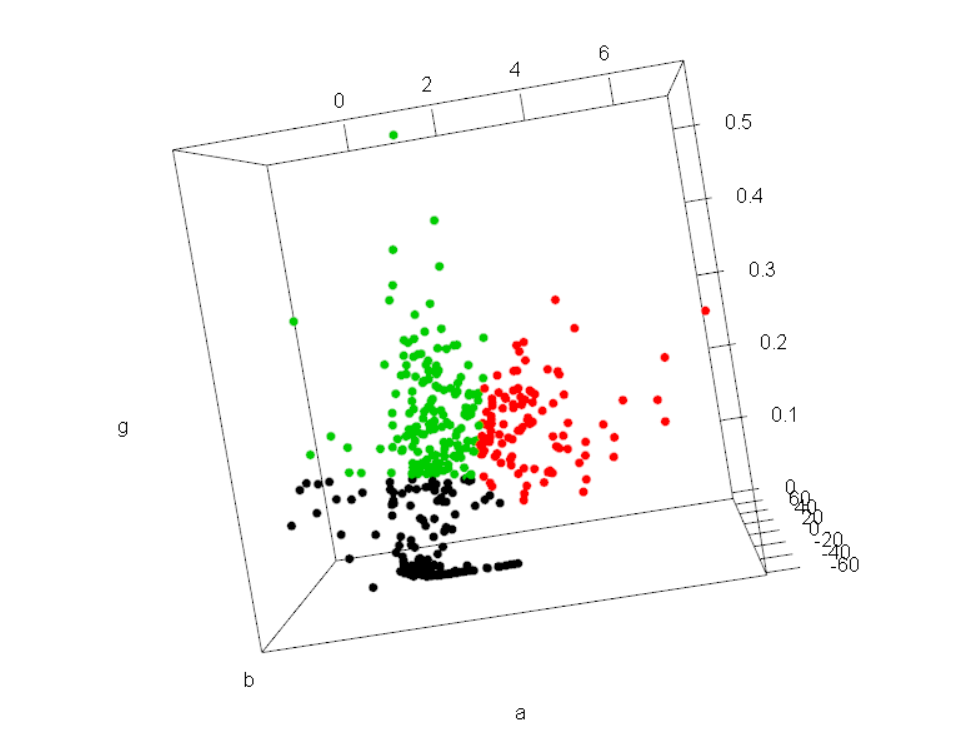
\includegraphics[scale=0.30]{Imagens/total}\par
\fonte{{\footnotesize (Os autores 2018)}}%
\end{center}
\end{figure}

Com as classificações realizadas pelo \textit{k-means} foi gerado o dataset para treinamento da rede neural. Na próxima seção serão apresentados os resultados obtidos.

\subsection{Classificação para diferentes Áreas de conhecimento realizadas com RNA}
Durante a fase de treinamento, a rede obteve um comportamento de erro aceitável, sendo necessário apenas alguns ajustes como descrito na seção 4. Após os ajustes necessários, foi obtido o gráfico de erro da rede ao longo das épocas como mostra a Figura 2.

\begin{figure}[h]
\caption{Erro da rede ao longo das épocas para rede treinada em diferentes áreas de conhecimento.}\label{fig2}\vspace{-0.5cm}
\begin{center}
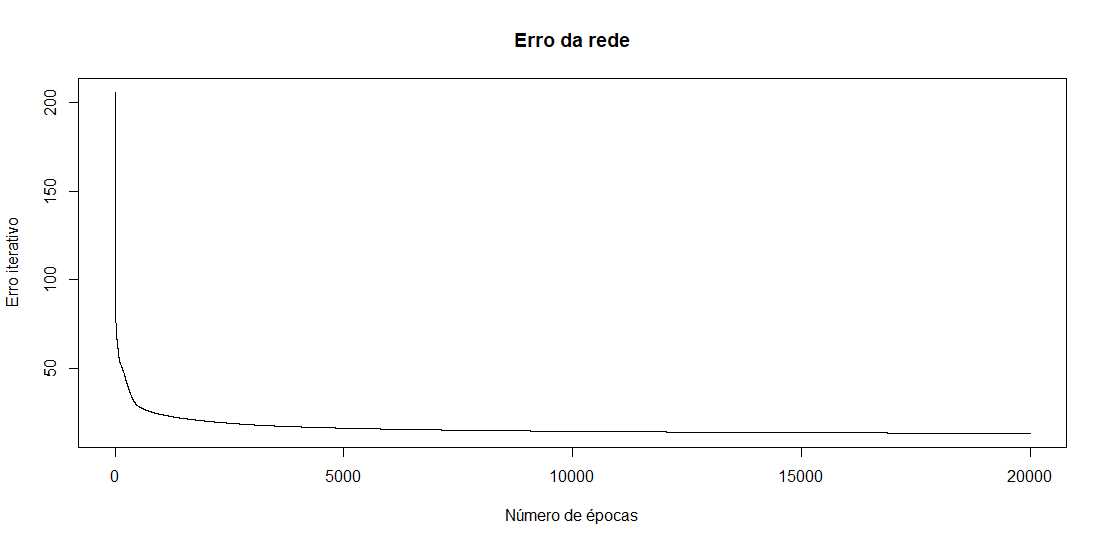
\includegraphics[scale=0.4]{Imagens/erro_Rede_diferentes_Areas}\par
\fonte{{\footnotesize (Os autores 2018)}}%
\end{center}
\end{figure}

Após treinada e ajustada, a rede classificou as questões do ENEM com base no \textit{dataset} das questões de diferentes áreas de conhecimento, como mencionado anteriormente. A fiura 3 ilustra a matriz de confusão gerada a partir da classificação da rede, onde a diagonal secundária representa os valores esperados e as demais, os erros da rede. Esses resultados mostram que as redes neurais são ferramentas poderosas para classificação de objetos em categorias distintas, Conforme é possível observar, a rede teve 86\% de acerto nas classificações realizadas mostrando ótimos resultados para classificação esperada das questões. 

\begin{figure}[h]
\caption{Matriz de confusão para questões de diferentes áreas de conhecimento.}\label{fig3}\vspace{-0.5cm}
\begin{center}
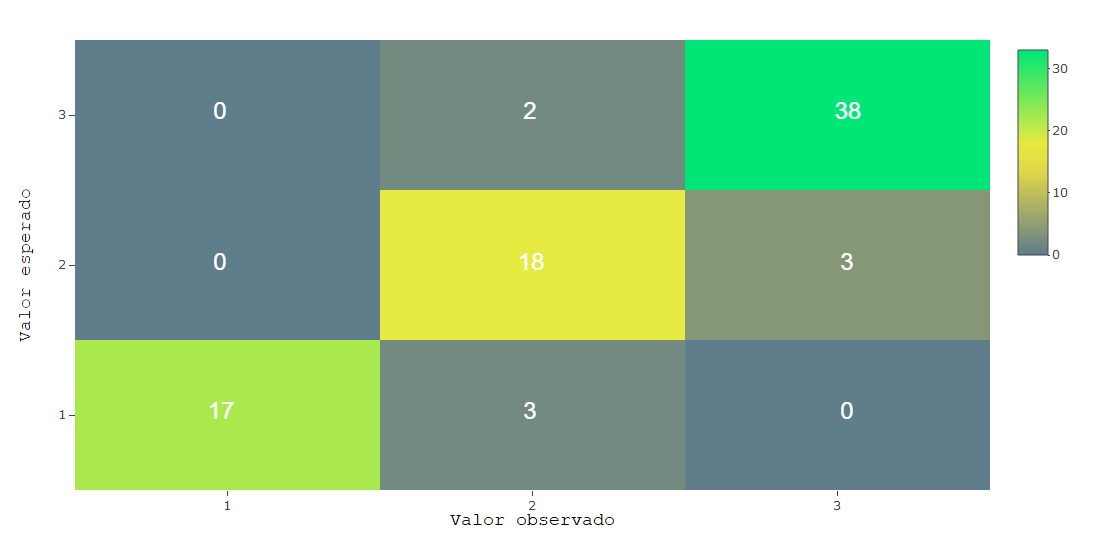
\includegraphics[scale=0.35]{Imagens/segunda_classf_matrix_todas_areas}\par
\fonte{{\footnotesize (Os autores 2018)}}%
\end{center}
\end{figure}

\subsection{Classificação para áreas únicas de conhecimento}
Foram criados novos experimentos de classificação com uma única rede para cada área de conhecimento. A taxa de erro em Ciêncas Humanas 100\%, em Ciências Naturais 96,29\% e em Matemática foi de 100\%. Estes resultados demonstram que redes neurais artificiais treinadas em um ambiente homogêneo possuem maior precisão de acerto quando utilizadas para classifcação. Os desempenhos das redes em cada um destes experimentos foram bastante similares, logo apenas o resultado de uma área será mostrado, sendo esta Ciências Humanas. Os resultados das demais áreas estão presentes no Apêndice. Sendo assim, as figuras 4 e 5 mostram respectivamente, o erro ao longo das épocas e a matriz de confusão gerada a partir da classificação realizada pela rede para área de Ciências Humanas. Conforme é possível observar a rede não teve nenhum erro durante a classificação.

\begin{figure}[h]
\caption{Erro da rede ao longo das épocas}\label{fig4}\vspace{-0.5cm}
\begin{center}
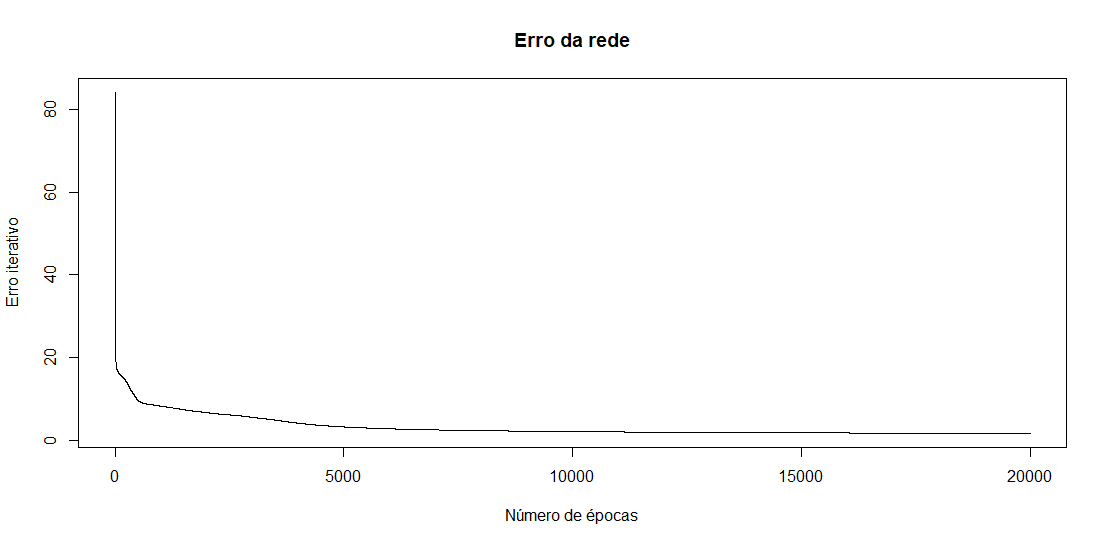
\includegraphics[scale=0.4]{Imagens/erroCH}\par
\fonte{{\footnotesize (Os autores 2018)}}%
\end{center}
\end{figure}

\begin{figure}[h]
\caption{Matriz de confusão para as questões de Ciências Humanas}\label{fig5}\vspace{-0.5cm}
\begin{center}
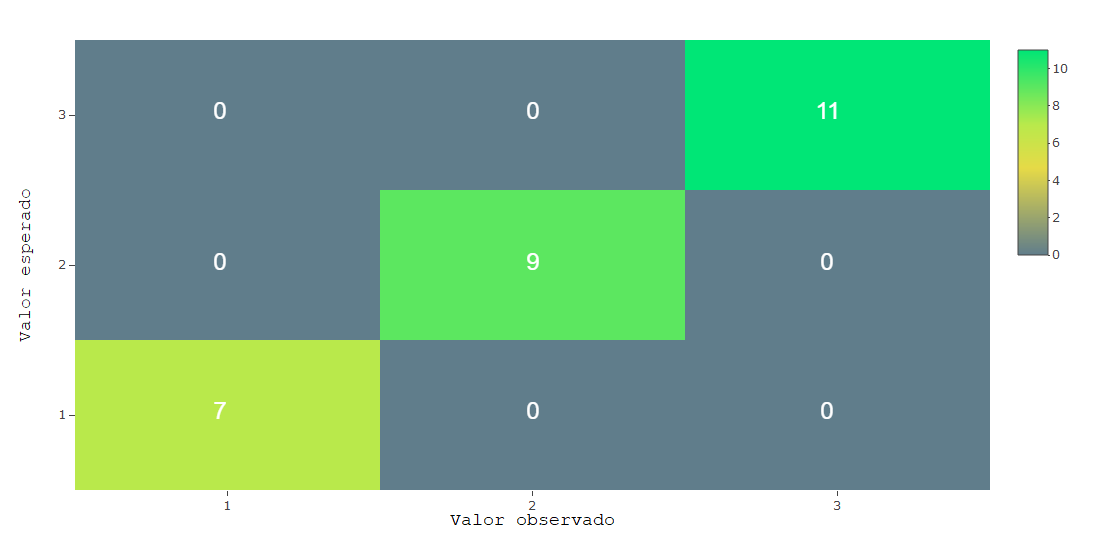
\includegraphics[scale=0.35]{Imagens/segunda_Classf_CH}\par
\fonte{{\footnotesize (Os autores 2018)}}%
\end{center}
\end{figure}

Comparando as matrizes de confusão geradas a partir da classificação de questões de diferentes áreas e de áreas únicas de conhecimento, é possível perceber que as redes treinadas para classificação de questões em uma única área obtiveram um melhor desempenho. O gráfico de erro ao longo das épocas não teve tanta diferença, contudo ainda é possível observar que a rede treinada em diferentes áreas do conhecimento converge um pouco mais devagar para zero se comparada com as outras redes.

Diante dos resultados obtidos com o presente trabalho, conclui-se que a utilização do algoritmo \textit{k-means} para classificações de questões do ENEM em grupos de dificulade é bem interessante em relação a seus resultados, todavia, o custo para realizar esta classifcação pode tornar o seu uso não viável dependendo da aplicação. As redes neurais mostraram ser uma boa alternativa ao \textit{k-means} para esse tipo de classificação, uma vez que seu custo de classificação é linear, enquanto o custo do \textit{k-means} para espaço e sementes fixas (\textit{d} e \textit{k} respectivamente) é de $\mathcal{O}(n^{dk+1})$.
\bibliography{referencias_abntex2}

\SingleSpacing % usado para garantir que o ABSTRACT fique com espaçamento SIMPLES entre linhas.

\begin{center}
\textbf{BEHAVIOR OF MLP ARTIFICIAL NEURAL NETWORKS FOR CLASSIFICATION OF TRI-BASED ENEM ISSUES}
\end{center}\vskip 0.5em                % Vertical space after title.

\begin{center}
\textbf{ABSTRACT}
\end{center}

\noindent The National High School Examination (ENEM) in Brazil gains each year more importance, replacing traditional vestibular. With this, the development of tools that help prepare students is of great importance. Many simulations are done in a practically random way, with questions chosen without criterion. In this context, this work presents the development of a neural network to classify ENEM issues, based on the parameters of Item Response Theory. For this, the \ textit {k-means} algorithm will be used to generate a \ textit {dataset} containing the classification of these questions into 3 groups: Easy, Medium and Difficult. With this \ textit {dataset} a neural network will be trained to sort the questions and verify the results. In this way this study contributes allowing the elaboration of simulated in a balanced way. In addition, after the network training the same will be able to perform the classification of new issues based on TRI. If k-means continued to be used the classification would have to be made again if new questions were added on the basis of questions. The developed network had practically the same performance as the k-means in the task of classification, this shows the capacity that the neural networks possess of classification.\par \vspace{1.0em}

\noindent\textbf{Keywords: } National School Examination in Brazil. Classification algorithms. Item Response Theory.

\end{document}
